\documentclass[slidestop,compress,mathserif]{beamer}
%\documentclass[slidestop,compress,mathserif,handout]{beamer}

%\documentclass[xcolor=dvipsnames,handout]{beamer}
%\documentclass[xcolor=dvipsnames]{beamer}

%\documentclass[handout]{beamer}

%%% To get rid of solutions on handouts:
\newcommand{\soln}[1]{\textit{\textcolor{darkGray}{#1}}}				% For slides
%\newcommand{\soln}[1]{ }	% For handouts

% to get pausing to work properly on slides
\newcommand{\hide}[1]{#1}	% For slides
%\newcommand{\hide}[1]{ }	% For handouts


%\usepackage{multicol}
\usepackage{amsfonts}
%\usepackage[pdftex,dvipsnames]{color}
\usepackage{graphicx}
\usepackage{subfigure}
%\usepackage{picinpar}
\usepackage{pifont}
\usepackage{pgf,pgfarrows,pgfnodes}
%\usepackage{wasysym,manfnt,phaistos,empheq}
\usepackage[english]{babel}
\usepackage{pgfpages}
\usepackage{natbib}
\usepackage{hyperref}
\usepackage{multimedia}
%\usepackage{amsfonts,amstext,amssymb,amsbsy,amsopn,amsthm,eucal,latexsym,mathrsfs}
\usepackage{amsmath,amsfonts,amstext,amssymb,amsbsy,amsopn,amsthm,eucal,latexsym,mathrsfs}
\usepackage{ulem}
\usepackage{setspace}
\usepackage{array}
%\usepackage{rotating}
\usepackage{multirow}
\usepackage{verbatim}
\usepackage{multicol}

\setbeamertemplate{navigation symbols}{}

%\usepackage{tikz}
%\usetikzlibrary{arrows,shapes,trees,backgrounds}


%\setbeameroption{show notes on second screen}
%\setbeameroption{show notes}
%\setbeameroption{show only notes}

\definecolor{links}{HTML}{2A1B81}
\hypersetup{colorlinks,linkcolor=,urlcolor=links}

\newtheorem*{principle}{Inscrutibility Principle}
\newtheorem*{punchline}{Punch Line}
\newtheorem{defn}{Definition}

\definecolor{Scarlet}{RGB}{140,17,17}
\definecolor{VassarRed}{RGB}{128,0,0}

% "dinglist" environment
  \renewenvironment{dinglist}[2][blue]
  {\begin{list}{\textcolor{blue}{\ding{#2}}}{}}{\end{list}}
  % Symbol definitions for these lists
  \newcommand{\DingListSymbolA}{43}
  \newcommand{\DingListSymbolB}{243}
  \newcommand{\DingListSymbolC}{224}
  \newcommand{\DingListSymbolD}{219}
  \newcommand{\DingListSymbolCheck}{52}
  \newcommand{\DingListSymbolCross}{56}


  \newenvironment{ballotenv}
{\only{%
\setbeamertemplate{itemize item}{\ding{45}}%
\setbeamertemplate{itemize subitem}{\ding{46}}%
\setbeamertemplate{itemize subsubitem}{\ding{46}}}} {}
\setbeamertemplate{itemize item}{\ding{49}}
\setbeamertemplate{itemize subitem}{\ding{47}}
\setbeamertemplate{itemize subsubitem}{\ding{47}}


%User defined colors: See colors section
\xdefinecolor{oiBlue}{rgb}{0.15, 0.35, 0.55}
\xdefinecolor{gray}{rgb}{0.5, 0.5, 0.5}
\xdefinecolor{darkGray}{rgb}{0.3, 0.3, 0.3}
\xdefinecolor{darkerGray}{rgb}{0.2, 0.2, 0.2}
\xdefinecolor{rubineRed}{rgb}{0.89,0,0.30}
\xdefinecolor{linkCol}{rgb}{0.11,0.49,0.95}	
\xdefinecolor{irishGreen}{rgb}{0,0.60,0}	
\xdefinecolor{darkturquoise}{rgb}{0.44, 0.58, 0.86}
\definecolor{lightGreen}{rgb}{0.533,0.765,0.42}
\xdefinecolor{Regalia}{HTML}{522D80}
\xdefinecolor{ClemsonOrange}{HTML}{EA6A20}

\definecolor{duke@LightGrey}{RGB}{200,200,200}\definecolor{DarkGreen}{RGB}{0,100,0}
\definecolor{Oranges}{RGB}{255,127,0}
\definecolor{LightGray}{RGB}{211,211,211}

%\setbeamertemplate{footline}{%
%  \raisebox{5pt}{\makebox[\paperwidth]{\hfill\makebox[10pt]{\scriptsize\insertframenumber}}}}

\setbeamercolor{equation background}{fg=black,bg=duke@LightGrey}
  % Boxed equation
  \newcommand{\eqbox}[2][0.6]{%
  \centerline{
  \begin{beamerboxesrounded}[lower=equation background,width=#1\hsize,shadow=true]{}
\parbox{#1\hsize}{%
      \[
        \textcolor{black} {#2}
      \]}
  \end{beamerboxesrounded}
}}

\AtBeginSection[] {
  \begin{frame}<beamer>\frametitle{Outline}
    \tableofcontents[currentsection,hideothersubsections]
  \end{frame}
}
%
%
%\AtBeginSubsection[] {
%  \begin{frame}<beamer>\frametitle{Outline}
%    \tableofcontents%[currentsection,currentsubsection]
%  \end{frame}
%}

%\usecolortheme[RGB={82,45,128}]{structure}
%\usecolortheme[RGB={162,80,22}]{structure}
\usecolortheme[RGB={128,0,0}]{structure}
\usetheme[secheader]{Boadilla}
%\usetheme[height=7mm]{Rochester}
%\usetheme{Copenhagen}
%\usetheme{Antibes}
%\usecolortheme{seahorse}
%\usecolortheme{crane}
%\usecolortheme{rose}
%\usefonttheme[onlylarge]{structurebold}
%\usefonttheme[onlymath]{serif}



\def\diag{{\rm diag}}


\def\E{\mathbb{E}}
\def\Prob{\mathbb{P}}
\def\argmin{{\rm argmin}}
\def\argmax{{\rm argmax}}
\def\Def{\stackrel{def}{=}}


\newtheorem{assumption}{Assumptions}
\newtheorem*{proposition}{Proposition}
\newtheorem*{remark}{Remark}



%\setbeamercolor{disc title}{bg=oiBlue!40!white!60,fg=blue}
\setbeamercolor{disc body}{bg= Regalia!20!white!80,fg= Regalia!80!black!90}

\setbeamercolor{clicker ungraded title}{bg=irishGreen!80!white!50,fg=irishGreen!30!black!90}
\setbeamercolor{clicker ungraded body}{bg=irishGreen!20!white!80,fg=irishGreen!30!black!90}

\setbeamercolor{clicker review title}{bg=gray!80!white!80,fg=oiBlue!80!black!90}
\setbeamercolor{clicker review body}{bg=gray!30!white!90,fg=oiBlue!80!black!90}

\setbeamercolor{code body}{bg=gray!20!white!80,fg=black}


% Custom commands
\newcommand{\degree}{\ensuremath{^\circ}}
\newcommand{\Note}[1]{
\rule{2.5cm}{0.25pt} \\ \textit{\scriptsize {\textcolor{rubineRed}{Note:} \textcolor{gray}{#1}}}}
\newcommand{\ct}[1]{
\vfill
{\tiny #1}}
\newcommand{\Remember}[1]{\textit{\scriptsize{\textcolor{orange}{Remember:} \textcolor{gray}{#1}}}}
\newcommand{\red}[1]{\textit{\textcolor{rubineRed}{#1}}}
\newcommand{\pink}[1]{\textit{\textcolor{rubineRed!90!white!50}{#1}}}
\newcommand{\green}[1]{\textit{\textcolor{irishGreen}{#1}}}
\newcommand{\webURL}[1]{\urlstyle{same}\textit{\textcolor{linkCol}{\url{#1}}} }
\newcommand{\webLink}[2]{\href{#1}{\textcolor{linkCol}{{#2}}}}
\newcommand{\mail}[1]{\href{mailto:#1}{\textit{\textcolor{linkCol}{#1}}}}
\newcommand{\hl}[1]{\textit{\textcolor{oiBlue}{#1}}}
\newcommand{\hlGr}[1]{\textit{\textcolor{lightGreen}{#1}}}
\newcommand{\mathhl}[1]{\textcolor{oiBlue}{\ensuremath{#1}}}
\newcommand{\ex}[1]{\textcolor{blue}{{{\small (#1)}}}}
\newcommand{\disc}[1]{
\begin{beamerboxesrounded}[shadow = true, lower = disc body, upper = disc title]{}
#1
\end{beamerboxesrounded}
}

\newcommand{\cl}[1]{
\begin{beamerboxesrounded}[shadow = true, lower = clicker ungraded body, upper = clicker ungraded title]{Question}
$\:$ \\
#1
\end{beamerboxesrounded}
}

\newcommand{\clR}[1]{
\begin{beamerboxesrounded}[shadow = true, lower = clicker review body, upper = clicker review title]{\red{Review question} }
$\:$ \\
#1
\end{beamerboxesrounded}
}

\newcommand{\formula}[2]{
\begin{beamerboxesrounded}[shadow = true, lower = white, upper = clicker review body]{#1}
#2
\end{beamerboxesrounded}
$\:$ \\
}

\newenvironment{twocol}[4]{
\begin{columns}[c]
\column{#1\textwidth}
#3
\column{#2\textwidth}
#4
\end{columns}
}


\newenvironment{slot}[2]{
\begin{array}{c}
\underline{#1} \\
#2
\end{array}
}

\newcommand{\pr}[1]{
\left( #1 \right)
}

\newcommand{\solnMult}[1]{
\item[] \vspace{-0.59cm}
\only<beamer| beamer:1>{\item #1}
\soln{\only<2->{\item \red{#1}}}
}

%\newcommand{\codechunk}[1]{
%\begin{beamerboxesrounded}[shadow = true, lower = code body]{}
%{\small #1}
%\end{beamerboxesrounded}
%}

% Change margin

\newenvironment{changemargin}[2]{%
\begin{list}{}{%
\setlength{\topsep}{0pt}%
\setlength{\leftmargin}{#1}%
\setlength{\rightmargin}{#2}%
\setlength{\listparindent}{\parindent}%
\setlength{\itemindent}{\parindent}%
\setlength{\parsep}{\parskip}%
}%
\item[]}{\end{list}}

% Footnote

\long\def\symbolfootnote[#1]#2{\begingroup%
\def\thefootnote{\fnsymbol{footnote}}\footnote[#1]{#2}\endgroup}

% Commands from the book
\newenvironment{data}[1]{\texttt{#1}}{}
\newenvironment{var}[1]{\texttt{#1}}{}
\newenvironment{resp}[1]{\texttt{#1}}{}








%%%%%%%%%%%%%%%%%%%%%%%%%%%%%%%%%%%%%%%%%%%%%%%%%%%%%%%%%%%%%%%%%%%%%%%%%%%%%%%%%%%%%%%%%%%%%%%

\title[MATH 241 Introduction]{MATH 241 Introduction}
%\subtitle{}

%%%%%%%%%%%%%%%%%%%%%%%%%%%%%%%%%%%%%%%%%%%%%%%%%%%%%%%%%%%%%%%%%%%%%%%%%%%%%%%%%%%%%%%%%%%%%%%


\author[Jingchen (Monika) Hu] % (optional, use only with lots of authors)
{Jingchen (Monika) Hu}
% - Give the names in the same order as the appear in the paper.
% - Use the \inst{?} command only if the authors have different
%   affiliation.

\institute[Vassar] % (optional, but mostly needed)
{Vassar College}
% - Use the \inst command only if there are several affiliations.
% - Keep it simple, no one is interested in your street address.

\date[MATH 241] % (optional, should be abbreviation of conference name)
{MATH 241}
% - Either use conference name or its abbreviation.
% - Not really informative to the audience, more for people (including
%   yourself) who are reading the slides online

\subject{MATH 241}
% This is only inserted into the PDF information catalog. Can be left
% out.



% If you wish to uncover everything in a step-wise fashion, uncomment
% the following command:

%\beamerdefaultoverlayspecification{<+->}


\begin{document}




%%%%%%%%%%%%%%%%%%%%%

% Title Page

%\begin{frame}%[plain]
%\titlepage
%\end{frame}

%%%%%%%%%%%%%%%%%%%%%
\addtocounter{framenumber}{-1}


%%%%%%%%%%%%%%%%%%%%%

%\begin{frame}{Outline}
%%\tableofcontents[hideallsubsections,pausections]
%\tableofcontents[hideallsubsections]
%\end{frame}

%%%%%%%%%%%%%%%%%%%%%
%%%%%%%%%%%%%%%%%%%%%

\section{Course topics}

%%%%%%%%%%%%%%%%%%%%%


\begin{frame}{Who am I?}
\begin{columns}
\column{.65\textwidth}
\vspace{-2cm}
\begin{itemize}
\item \textbf{Jingchen (Monika) Hu}
\vspace{0.5cm}
\item Joined Vassar in 2015
\begin{itemize}
\item Ph.D.\ in Statistics, Duke University, Durham, NC 
%\item Master in Statistics, Duke University
\item B.S.\ in Computing Mathematics, City University of Hong Kong, China 
\end{itemize}
\vspace{0.5cm}
\item Research and teaching interests:
\begin{itemize}
\item Bayesian statistics (MATH 347)
\item Data confidentiality: class survey example (Intensive Spring 2020)
% \item Imputation for missing data
\item I love teaching MATH 241! This is my 4th time to teach this class.
\end{itemize}
\end{itemize}
\column{.35\textwidth}

\includegraphics[width=2.1cm,height=2.1cm]{figures/vassar-logo.png}
\vspace{0.5cm}

\includegraphics[width=2.1cm,height=2.2cm]{figures/duke-logo.png}
\vspace{0.5cm}

\includegraphics[width=4.1cm,height=2.2cm]{figures/cityu-logo.jpg}
\end{columns}

\end{frame}

\begin{frame}\frametitle{Who are you all? }

\begin{itemize}
\item Introduce yourself to your neighbor (name, year, major/correlate)

\item Why are you taking MATH 241 Probability?

\item What you want to get out of MATH 241 Probability?
\end{itemize}

\end{frame}


\begin{frame}\frametitle{One question for you!}

\disc{Draw two socks at random, without replacement, from a drawer full of twelve colored socks:
\vspace{-0.3cm}
\begin{center}
6 black, 4 white, 2 purple
\end{center}
Let $B$ be the number of Black socks, $W$ the number of White socks drawn.
}
Then the distributions of $B$ and $W$ are given by:

\uncover<2->{
\begin{center}
\renewcommand{\arraystretch}{2}
\begin{tabular}{c|c|c|c|}
       & 0                                           &1                                            & 2                                           \\
\hline
$P(B=k)$ & \uncover<3->{$\frac{6}{12} \cdot\frac{5}{11} = \frac{15}{66}$}  &  \uncover<4->{$2\cdot\frac{6}{12} \cdot\frac{6}{11} = \frac{36}{66}$} &  \uncover<5->{$\frac{6}{12}\cdot \frac{5}{11} = \frac{15}{66}$} \\
\hline
$P(W=k)$ &\uncover<6->{$\frac{8}{12} \cdot\frac{7}{11} = \frac{28}{66}$} &  \uncover<7->{$2\cdot\frac{4}{12}\cdot \frac{8}{11} = \frac{32}{66}$} & \uncover<8->{$\frac{4}{12} \cdot\frac{3}{11} = \frac{6}{66}$}  \\
\hline
\end{tabular}
\end{center}

\uncover<9->{\footnotesize
Formally - $P(B=k)  = \frac{ {6 \choose k} {6 \choose 2-k} }{ {12 \choose 2} }$ and $P(W=k) = \frac{ {4 \choose k} {8 \choose 2-k} }{ {12 \choose 2} }$\\
{\color{VassarRed}Combinatorial Analysis (Chapter 1) \& Axioms of Probability (Chapter 2)}
}

}
\end{frame}


\begin{frame}\frametitle{Another question for you!}

\disc{Draw two socks at random, without replacement, from a drawer full of twelve colored socks:
\vspace{-0.3cm}
\begin{center}
6 black, 4 white, 2 purple
\end{center}
Let $B$ be the number of Black socks, $W$ the number of White socks drawn.
}
Then the distributions of $B$ and $W$ are given by:


\begin{center}
\renewcommand{\arraystretch}{2}
\begin{tabular}{c|c|c|c|}
       & 0                                           &1                                            & 2                                           \\
\hline
$P(B=k)$ & {$\frac{6}{12} \cdot\frac{5}{11} = \frac{15}{66}$}  &  {$2\cdot\frac{6}{12} \cdot\frac{6}{11} = \frac{36}{66}$} &  {$\frac{6}{12}\cdot \frac{5}{11} = \frac{15}{66}$} \\
\hline
$P(W=k)$ &{$\frac{8}{12} \cdot\frac{7}{11} = \frac{28}{66}$} &  {$2\cdot\frac{4}{12}\cdot \frac{8}{11} = \frac{32}{66}$} & {$\frac{4}{12} \cdot\frac{3}{11} = \frac{6}{66}$}  \\
\hline
\end{tabular}
\end{center}

{\footnotesize
What's the probability of $B = 0$ {\color{red}and} $W = 0$ (i.e. $P(B=0, W=0)$)? \\ \pause
What's the probability of $W=0$ {\color{red}given} that we know $B=0$ (i.e. $P(W=0 \mid B=0)$)?\\
{\color{VassarRed}Jointly Distributed Random Variables (Chapter 6)}
}


\end{frame}


\begin{frame}\frametitle{One more question for you! - last one, I promise}

\disc{Let X and Y have independent Uniform$(0, 1)$ distribution. Find the distribution of $X+Y$.}

\pause

\begin{center}
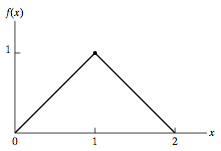
\includegraphics[width=0.35\textwidth]{figures/triangle_density}
\end{center}

\begin{align*}
f_{X+Y}(z)   =  \begin{cases}
              z & \text{if $0<z\leq1$} \\
              2-z & \text{if $1<z<2$}\\
              0 & \text{otherwise}
              \end{cases}
\end{align*}

{\color{VassarRed}Jointly Distributed Random Variables (Chapter 6)}



\end{frame}


\begin{frame}\frametitle{Topics to cover}
\begin{itemize}

\item Chapter 1 Combinatorial Analysis
\begin{itemize}
\item Permutations \& Combinations, Binomial \& Multinomial coefficients
\end{itemize}

\item Chapter 2 Axioms of Probability
\begin{itemize}
\item Sample space and events, axioms of probability
\end{itemize}



\item Chapter 3 Conditional Probability and Independence
\begin{itemize}
\item Conditional probabilities, Bayes' formula, independent events
\end{itemize}

{\bf \large {\color{VassarRed}Midterm I, week of 3/21 - 3/28, take-home open-book open-notes.}}

\pause

\item Chapter 4 (Discrete) Random Variables
\begin{itemize}
\item Expectation \& variance (sum), Bernoulli, Binomial, Poisson, Geometric
distributions, NY quick draw game
\end{itemize}

\item Chapter 5 Continuous Random Variables
\begin{itemize}
\item Expectation \& variance (integral), Uniform, Normal, Exponential,
Gamma distributions
\end{itemize}

\end{itemize}

\end{frame}



\begin{frame}\frametitle{Topics to cover cont'd}
\begin{itemize}

\item Chapter 6 Jointly Distributed Random Variables
\begin{itemize}
\item Joint distribution, independent random variables, sum of IRV,
conditional distribution
\end{itemize}

{\bf \large {\color{VassarRed}Midterm II, week of 5/3 - 5/10, take-home open-book open-notes.}}

\pause


\item Chapter 7 Properties of Expectation
\begin{itemize}
\item Properties of expectation, covariance and correlation, moment
generating functions
\end{itemize}


\item Chapter 8 Limit Theorems
\begin{itemize}
\item Markov's and Chebyshev's inequalities, Central Limit Theorem (CLT)
and law of large numbers (LLN)
\end{itemize}

{\bf \large {\color{VassarRed}Final exam, TBA.}}

\end{itemize}

\end{frame}



%%%%%%%%%%%%%%%%%%%%%
%%%%%%%%%%%%%%%%%%%%%

\section{Syllabus \& policies}


%%%%%%%%%%%%%%%%%%%%%
\begin{frame}
\frametitle{General Info}

\begin{tabular}{ p{3cm} p{9cm} }
\textbf{Classroom:}		& Zoom \\
\textbf{Time:}			& Section 01: TTh 9:00am - 10:15am \\
					& Section 02: TTh 10:30am - 11:45am \\
					& \\
\textbf{Instructor:}		& Jingchen (Monika) Hu \href{mailto:jihu@vassar.edu}{\textit{jihu@vassar.edu}} \\
\textbf{Office:}			& Zoom\\
\textbf{Office hours:}		&  Tuesdays 10:00am - 11:30am \\
					& Wednesday 10:00am - 11:30am \\
					& or by appointment (link on Moodle) \\
					& \\
\textbf{Textbook:}		& A First Course in Probability, 9$^{th}$ Edition\\
					& Sheldon M. Ross, Prentice Hall\\					
\textbf{Website:}		& Moodle (course material: slides and homework etc.)\\
 &Google Drive (schedule and surveys etc.) and Slack\\%\hl{\webURL{TBD}}\\
\textbf{Workload:}		& On average 6-8 hours every week outside of class\\
					
\end{tabular}

\end{frame}

%%%%%%%%%%%%%%%%%%%%%%%%%%%%%%%%%%%%






%%%%%%%%%%%%%%%%%%%%%%%%%%%%%%%%%%%%

\begin{frame}
\frametitle{Grading}

\begin{center}
\begin{tabular}{l l }%p{0.5cm} l l p{0.5cm} l l}
Homework 	& 15\%	\\
Quizzes 	& 10\%	\\
Weekly check-ins and team work solutions & 10\% \\
Midterms (20\% $\times$ 2) 	& 40\%	\\
 Final Exam		& 25\%	
\end{tabular}
\end{center}

\pause
\begin{itemize}
\item Grades curved at the end of the course after overall averages have been calculated.
\begin{itemize}
\item Average of 90-100 guaranteed A-.
\item Average of 80-90 guaranteed B-.
\item Average of 70-80 guaranteed C-.
\item Average of 60-70 guaranteed D-.
\end{itemize}
\item The more evidence there is that the class has mastered the material, the more generous the curve will be.
\end{itemize}


\end{frame}

%%%%%%%%%%%%%%%%%%%%%%%%%%%%%%%%%%%%

\begin{frame}
\frametitle{General course schedule}

\begin{itemize}
\item Fully remote.

\item Recorded lectures (no class on Tuesdays).

\item Live sessions, work in teams (every Thursday).

\item Weekly check-ins due every Sunday 11:59pm EST.

\item Homework due Sunday 11:59pm EST (in the week it is due).

\item Quizzes in-class on Thursdays.

\item My office hours: Tuesdays 10:00 - 11:30am \& Wednesdays 10:00 - 11:30am, or by appointment. 

\item I also check our Slack channel at least once a day - ask me or your fellow students any questions you have on Slack!
\end{itemize}
\end{frame}

\begin{frame}
\frametitle{Recorded lectures}

\begin{itemize}
\item Roughly 5 - 8 recorded lectures for each week.

\item Available before Monday when a week starts.

\item Lecture slides for recorded lecture videos posted on Moodle.
\end{itemize}

\end{frame}


\begin{frame}
\frametitle{Live sessions}

\begin{itemize}
\item Every Thursday during scheduled class meeting time (required).

\item Students work in teams.

\item A list of exercises will be posted before session starts.

\item Each team is responsible to provide solutions to one exercise by Sunday 11:59pm EST, Moodle submission.

\item I will provide my solutions after students' submission.

\item Students receive a participation grade
	\begin{itemize}
	\item attending live session
	\item work in teams
	\item submit team solutions (each student needs to make a submission on Moodle)
	\end{itemize}
\end{itemize}
\end{frame}
%\begin{frame}
%\frametitle{Lectures and short instructional videos}
%
%Three versions of slides for each chapter will be posted on Moodle.
%\begin{itemize}
%\item Pre-class version: posted before the lecture.
%Students are highly encouraged to print the pre-class slides out,
%bring them to class and take notes on them.
%\item In-class and handout versions: posted after completing
%each chapter.
%\end{itemize}
%
%\pause \vfill
%
%Short instructional videos.
%\begin{itemize}
%\item Before each lecture, you are expected to watch a short (about 5 minutes) instructional video covering the definition (and a simple example/exercise) of a new concept. 
%\item In class, we will work in groups to practice solving more complicated problems.
%\item Feel free to bring any interesting and relevant questions to class!
%\end{itemize}
%%\pause \vfill
%%
%%In-class questions (1\% overall grades):
%%\begin{itemize}
%%\item Questions in green frames: derivation, calculation, and (occasionally) multiple choice questions.
%%\item Students are randomly drawn to answer them.
%%\item Get credit for accuracy.
%%\end{itemize}
%
%
%
%\end{frame}
%


%%%%%%%%%%%%%%%%%%%%%%%%%%%%%%%%%%%%

\begin{frame}
\frametitle{Homework}

\begin{itemize}

\item About 8 homework assignments.

\item Due Sunday 11:59pm in the week it is due. 

\item Posted on Moodle for the week it is due (cover page and questions).
%\item Your homework must be stapled with the cover page.
%On the cover page, you must write your name, and you may list the questions you hope to be explained in class.

\pause
\item Show all your work to receive credit. Turn in your own work.

\item No make-ups.

\item Dispute about the grading has to be filed within one week after they are returned.

\item Answer keys to homework will posted on Moodle after the homework is due.
\pause

\item Late homework policy:
\begin{itemize}
%\item at the end of the class: lose 10\% of points
%\item late but on due date: lose 20\% of points
\item next day: lose 30\% of points
\item later than next day: lose all points
\end{itemize}

\end{itemize}

\end{frame}

%%%%%%%%%%%%%%%%%%%%%%%%%%%%%%%%%%%%

\begin{frame}
\frametitle{Quizzes}

\begin{itemize}

\item About every other week.

\item In-class on Thursdays, about 10-15 minutes.

\item Open-book and open-notes.

\item Date and topics will be announced in advance.

%\item Practice quizzes will be posted on BB randomly.


\pause
%\item Quizzes on the same day of excused absences (should be approved by me in advance) will be waived.

\item No make-ups for any quiz missed unless discussed beforehand.
\pause

%\item Extra credit for quizzes:  you are allowed to correct for quizzes after they are graded and returned. If correct, I will add back 25\% of the points you missed.

\end{itemize}

\end{frame}

%%%%%%%%%%%%%%%%%%%%%%%%%%%%%%%%%%%%


\begin{frame}
\frametitle{Weekly-check-ins}

\begin{itemize}
\item Every week.

\item Due Sunday 11:59pm EST, starting from this week.

\item Link on Moodle.

\item Students earn participation grade after completing each weekly check-in.
\end{itemize}

\end{frame}

%%%%%%%%%%%%%%%%%%%%%%%%%%%%%%%%%%%

\begin{frame}
\frametitle{Exams}
{\footnotesize
\begin{itemize}

\item Midterm I: \hl{week of 3/21 - 3/28}, take-home open-book open-notes.
\item Midterm II: \hl{week of 5/3 - 5/10}, take-home open-book open-notes.\\

%For both midterms, you will come in for a 1.5-hour exam during a 2.5-hour window from 6:00pm-8:30pm (you will choose from 3 possible start times: 6:00pm, 6:30pm, or 7:00pm). %Midterm II has a take-home portion which you will get after you finish the written exam.

\item Final: \hl{TBA by Registrar, during finals week}, take-home open-book open-notes.
%\item Closed book exams. You are allowed to bring a calculator and one sheet of notes (``cheat sheet") prepared by yourself.


\pause
\item No make-up for missed exams.
%\item Final exam grade will be used for the missed midterm exam if absence is excused.
\item {\footnotesize For the students who have at least 2 other final exams on the same day,
notify me at least one week before the final exam day so that I can accommodate your schedule individually.}

%\pause
%\item {\footnotesize Extra credit for midterm exams: within one week after you receive the graded exam, you may make a 10-minute appointment with me to re-do up to three problems {\bf orally}. If correct, I will add back 25\% of the points you missed in those questions.}
%


\end{itemize}

}

\end{frame}


%%%%%%%%%%%%%%%%%%%%%%%%%%%%%%%%%%%%

\begin{frame}
\frametitle{Other policies}

\begin{itemize}


\item All regrade requests on homework, quizzes and exams must be discussed with the instructor within one week of receiving your grade.
\item There will be no grade changes after the final exam.

%\pause
%
%\item Laptops, tablets, cell-phones, and any other electronic devices are not allowed in-class. % (unless I let you).
%\item Food is not allowed in class.
%
%\pause
\item Academic integrity


\end{itemize}

\end{frame}

%%%%%%%%%%%%%%%%%%%%%

\begin{frame}
\frametitle{Tips for success}

\begin{enumerate}
\item Do the homework - start early.
\item Read the relevant sections before class, and review after the lectures.
\item Watch the assigned instructional videos, and rewatch them if necessary.
\item Be an active participant during lectures.
\item Ask questions - during class or office hours.
\item Prepare good cheat sheets for exams.
\item Do not procrastinate.
\end{enumerate}

\end{frame}



\begin{frame}\frametitle{Announcement}

\begin{itemize}
\item Class survey: \red{due Sunday 2/21}\\
Moodle course page $\longrightarrow$ Class survey\\

\item Weekly check-in for week 1: \red{due Sunday 2/21}\\
Moodle course page $\longrightarrow$ Week 1 (2/17 - 2/21) $\longrightarrow$ weekly check-in\\

\item HW1: \red{due Sunday 2/28}\\
Moodle course page $\longrightarrow$ Week 2 (2/22 - 2/28) $\longrightarrow$ Homework 1\\




\end{itemize}

\end{frame}



%%%%%%%%%%%%%%%%%%%%%%%%%%%%%%%%%%%%







\end{document}
